\documentclass[a4paper]{article}
\usepackage{graphicx}
\usepackage[utf8]{inputenc}
\usepackage[english, serbian]{babel}
\usepackage{comment}

\title{MATF Elektronski časopis}
\date{2018}
\author{Dimitrije Špadijer, Božidar Antić, Nadežda Bogdanović}


\begin{document}
\maketitle
\newpage
\tableofcontents
\newpage

\section{Cilj projekta}

Razviti veb platformu koja će omogućiti sve neophodne funkcionalnosti za uređivanje elektronskog časopisa. Časopis izlazi dva puta godišnje i tematski je organizovan. Jezik časopisa je engleski.

\section{ Analiza sistema}

\subsection{Učesnici}

    Atributi: id, ime, prezime, korisničko ime, šifra, institucija, email, telefon(opciono), poštanski broj(opciono)
    Korisnici sistema imaju mogućnost upravljanja sopstvenim nalogom (promena korisničkog imena i šifre). Korisnici se međusobno razlikuju po ulogama i privilegijama koje su im dodeljene: Administrator, glavni urednik, urednik, recenzent, autor

    \subsubsection{Administrator}
    Administrator je korisnik sistema koji upravlja podešavanjima sistema: dodele korisničkih imena i šifara, dodavanje i uklanjanje novih korisnika, upravljanje nalozima, održavanje sistema - dakle stvari tehnološke prirode. On se odmah od početka korišćenja sistema nalazi u bazi podataka - ne registruje se. Iako su mu vidljivi svi podaci o svim korisnicima, radovima i brojevima časopisa, nema pravo dodele uloga (urednika i recenzenata), osim u slučaju dodele uloge glavnom uredniku.

    \subsubsection{Glavni urednik}
    Na vrhu piramide odlučivanja. Ne registruje se u sistem, administrator ga dodaje. Prilikom prijavljivanja prikazuje mu se u prvom delu prozora spisak novo-prijavljanih radova u sistemu označenih na upadljiv način. U drugom delu rada nalazi se paleta za pretraživanje: po autoru, imenu rada, datumu, statusu rada, statusu urednika, statusu autora.. Odabirom autora prikazuju mu se informacije o autoru. Odabirom rada prelazi se na radni prostor u kojem se ispisuje: naziv rada i informacije o autorima (ime, prezime, status svakoga od njih). Sam rad se nalazi u prilogu. G.urednik ima opciju da: rad odbaci bez konsutovanja sa ostalima i da rad prosledi uredniku. Iz padajuće liste bira urednika kojem šalje rad, u suprotnom, rad se arhivira kao odbačen. Glavni urednik ima pravo i da dodeli recenzente, urednike i da odluči koji će se rad objavljivati u kojem broju, da doda autora na crnu listu. Ima pristup odeljku "Upravljanje korisnicima" u kojem može da dodeli uloge urednicima/recenzentima, ili da ih oduzme. Takođe ima mogućnost ostavljanja komentar na rad kada hoće da ga izmeni ili odobri/odbaci bez recenzije. On odlučuje koji će se radovi naći u kojem broju.

    \subsubsection{Urednici}
    Urednici su specijalizovani za određene oblasti (oblast se pridodaje kao atribut). Primaju od g.urednika rad, čitaju ga i šalju predloge recenzentima. Urednik ima pravo da odbaci/prihvati rad, iako recenzenti misle da je rad za objavljivanje, ali onda treba da napiše obrazloženje. Ako urednik misli da je radu potrebna neka izmena, ima opciju da rad označi za menjanje, označava ga i otvara mu se polje gde unosi komentar urednika, koji objašnjava šta je sve potrebno promeniti. Ako komentar  na rad već postoji, on se učita u prostor za pisanje komentara i urednik ga menja ili briše i dodaje novi. Komentar urednika je opciona stavka. Po istom principu funkcionište i odbijanje/prihvatanje bez recenzije. Urednik prilikom logovanja na sistem ima u gornjem delu prozora spisak novih radova koje mu je poslao g.urednik. U donjem delu prozora je paleta za pretraživanje, opisana kao kod g.urednika. Odabirom na novi rad urednik ga ili odbaci, ili mu dodeli recenzente.

    \subsubsection{Recenzenti}
    Prilikom logovanja imaju spisak novih radova poslatih od urednika. Rad mogu da odbiju, i dalje nemaju više nikakva zaduženja vezana za taj rad. Takođe, mogu da pristupe i spisku svih dosadašnjih radova: prihvaćenih i odbijenih. Nakon pročitanog rada, recenzent popunjava formular za recenziju i objavljuje je. Potencijalni recenzent je onaj koji: je već recenzirao neki rad, ko je  kao korisnk čekirao polje "nemam ništa protiv da me kontaktirate za recenziranje nekog rada"

    \subsubsection{Autori}
    Dodatni atributi: broj dosadašnjih prilaganja radova, broj dosada objavljenih radova. Postoji i crna lista nepoželjnih autora koja sadrži ime autora i razlog zbog kog se nalazi na listi:  plagiranje, različiti vidovi varanja utvrđeni od strane ostalih korisnika sistema. Autori prijavljuju rad. Prilikom prijave ispunjavaju formular i označavaju da li je to novi rad, ili nova verzija rada koji je označen za ispravku. Ako u nekom trenutku žele da povuku rad, šalju zahtev za povlačenje rada.

\subsection{Časopis}
Atributi: ISSN, godina, naslov, g.urednik, urednici, minimalan i maksimalan broj radova po izdanju

\subsection{Rad}
    Atributi: broj, naslov, godina, imena autora, datum prve prijave, datum poslednje prijave, log prijava, rad u pdf formatu, recenzenti, urednik, status, broj verzija, objavljen

    Statusi rada:
    \begin{itemize}
        \item prijavljen: dobija status kada ga autor prijavi
        \item na recenziji: kada ga primi recenzent na recenziju
        \item na doradi: ovaj status dobija kada ga g.urednik/urednik označi da treba da ide na doradu
        \item povučen: ako je autor podneo zahtev za povlačenje rada
        \item odbijen bez recenzije: od strane g.urednika/urednika. U tom slučaju je potrebno priložiti komentar (funkcioniše isto kao kada se rad označava za doradu). Rad je odbijen bez recenzije i ako urednik nije mogao da pronađe recenzente koji žele da recenziraju rad, a sam nije želeo da čita ceo rad
        \item odbijen sa recenzijom
        \item prihvaćen bez recenzije: slično kao odbijen bez recenzije, potrebno je ostaviti komentar
        \item prihvaćen sa recenzijom
    \end{itemize}


\begin{figure}[hbt!]
    \centering
    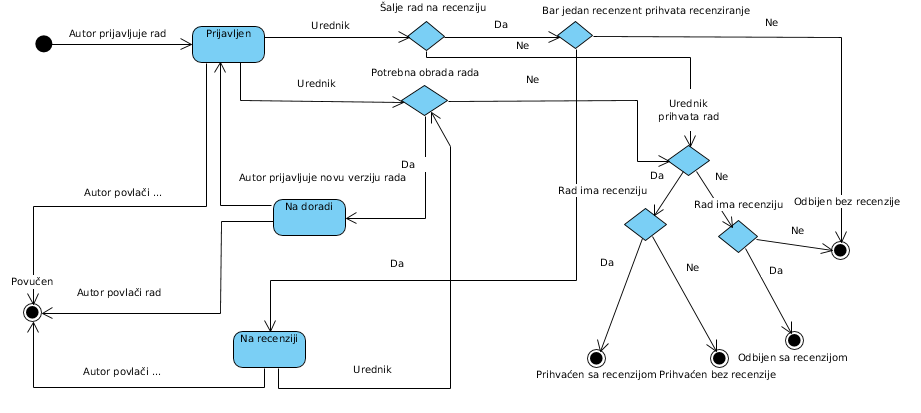
\includegraphics[width=1\linewidth]{StanjeRada.PNG}
    \caption{Stanja rada}
    \label{fig:my_label}
\end{figure}


\subsection{Prijavljivanje i registrovanje korisnika}
Prilikom registrovanja, korisnik ima mogućnost da označi opciju "nemam ništa protiv ako želite da me odaberete kao recenzenta". Ako ovu opciju nije čekirao, može to da učini kasnije kada se prijavi.
\begin{itemize}
    \item Registrovanje: popuni se formular i pošalju podaci. Administrator ih prima i šalje šablon1 u kojem korisnika obaveštava koje mu je korisničko ime i šifra
    \item Prijavljivanje: korisnik popuni formular i time se uloguje
\end{itemize}

\subsection{Komunikacija među korisnicima}
Korisnik odabere šablon, otvori mu se radna površina za pisanje u koju se šablon učita. On taj šablon može sačuvati i ima opciju da ga pošalje, čime se šablon automatski šalje na mejl drugog saučesnika u komunikacji. Korisnik može i napraviti novi šablon i obrisati ga, ako nije predefinisan od strane sistema, kao što su dole navedeni šabloni.


\begin{figure}[hbt!]
    \centering
    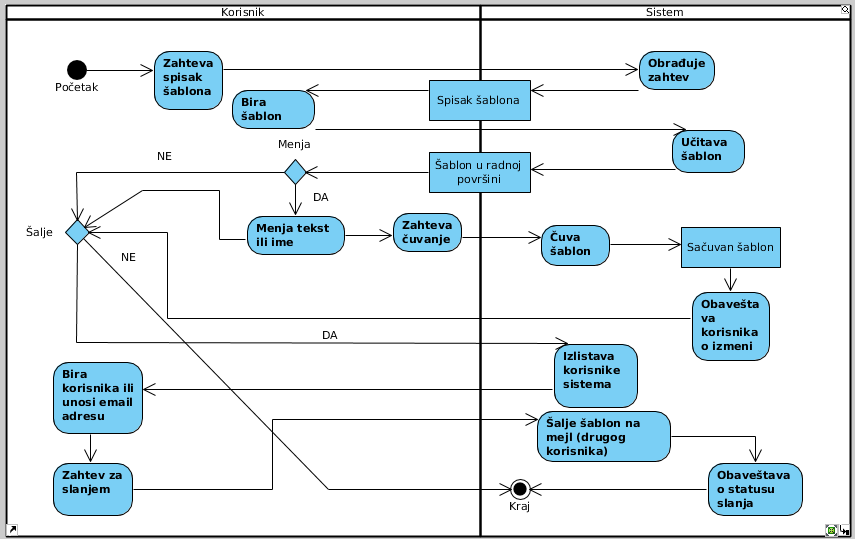
\includegraphics[width=\linewidth]{KomunikacijaMedjuKorisnicima.PNG}
    \caption{Komunikacija Među Korisnicima}
    \label{fig:my_label}
\end{figure}


\begin{itemize}
\item Administrator ostalim korisnicima: šabloni 1 (uspešno registrovanje) i 2 (uspešna/neuspešna promena ličnih podataka)
\item G.urednik urednicima: šablon 3 (o novopristiglom radu)
\item G.urednik administratoru: šablon 4 (o brisanju korisnika iz sistema)
\item Urednik recezentima: šablon 5 (predlog rada za recenziranje)
\item Urednik autoru: šablon 6 (o tome kako je rad prihvaćen i šta treba da priloži) i  šablon 7 (odbijen i obrazloženje)
\item Recenzent uredniku: šablon 7 (o tome da li odbija ili prihvata recenziju)
\item Šablon 8 sistem šalje autoru kada (glavni) urednik ostavi komentar na rad koji je napisao.
\end{itemize}

\begin{figure}[hbt!]
    \centering
    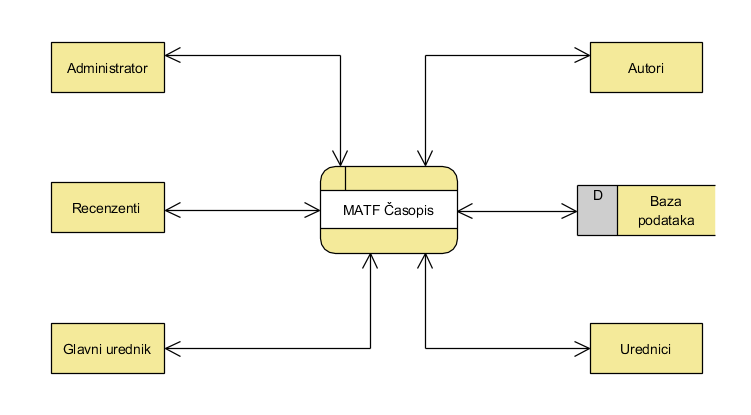
\includegraphics[width=1\linewidth]{Konteksta.PNG}
    \caption{Dijagram konteksta}
    \label{fig:my_label}
\end{figure}



\subsection{Životni ciklus rada}
\subsubsection{Prijavljivanje}
Rad prijavljuje autor koji je ujedno i odgovorno lice za taj rad. Spisak autora koje rad sadrži kao atribut mogu biti reference na autore već poznate sistemu, inače o autoru će biti napravljen zapis u sistemu koji će biti moguće koristiti kao njegov kontakt u slučaju da je to potrebno (npr. poziv za učlanjenje).
\subsubsection{Dodeljivanje urednicima i recenzentima}
Rad je inicijalno prikazan glavnom uredniku koji ga dodeljuje uredniku. On zatim "nudi" rad recenzentima koji imaju mogućnost da prihvate ili odbiju tu ulogu. Obaveštenja o dodelama radova i ponudama recenzentskih uloga su realizovana putem slanja šablona (opisanim u delu 6) i praćena su akcijama sistema.
\subsubsection{Recenziranje}
Sa spiska svih recenzenata u sistemu, urednik odabira recenzenta, koji se automatski dodeljuje kao recenzent datom radu i šalje mu se obaveštenje o tome. Kada se prijavi na sistem, prijavljuje mu se spisak svih novih radova za koje je predložen. Ako želi da recenzira rad, on može odmah nastaviti da piše recenziju, a ako ne, može odabrati opciju "Ne želim da recenziram ovaj rad", čime ga sistem automatski uklanja sa spiska recenzenata za taj rad i uredniku se šalje poruka koja ga obaveštava o tome.Od recenzenta se, ako je prihvatio recenziranje, očekuje da popuni formular koje će sadržati delove koji su upućeni autoru i uredniku. Nakon objavljivanja, uredniku su vidljiva oba dela, a autoru samo deo namenjen njemu.
\subsubsection{Komentarisanje rada}
Rad može biti komentarisan od strane glavnog urednika i urednika i to u slučajevima kada je rad odbijen sa komentarom, koji će autor moći da pročita kao objašnjenje za preduzetu akciju, ili kada se rad označava za doradu, čime se autoru stavlja do znanja koje su to promene koje se zahtevaju.
\subsubsection{Ažuriranje}
Nakon što je rad od strane urednika označen za doradu, autor ima mogućnost da izmenjenu verziju rada ponovo prijavi. U tom slučaju potrebna je ponoviti i dodelu recenzenata. Kao u slučaju prvobitne dodele, uredniku je ponuđen spisak recenzenata na kome bi favorizovani bili oni koji su na tom radu već imali recenzentsku ulogu.
\subsubsection{Menjanje statusa}
Status rada je inicijalno postavljen na "prijavljen" i može biti promenjen akcijama korisnika sistema. Moguća stanja i akcije koje dovode do tih stanja su navedene u delu 2.3.


\subsection{Sistemska podešavanja}
Obavlja ih administrator: upravljnje podacima u bazi, dodavanje novih korisnika i uklanjanje postojećih... Na nivou sistema treba da postoji log svih aktivnosti koji treba da bude vidljv administratoru i glavnom uredniku

\subsection{Šabloni i formulari}
Sadržaj šablona i formulara biće priložen nezavisno od ovog dokumenta u odeljku "Prilozi (Attachments)"



\begin{figure}[hbt!]
    \centering
    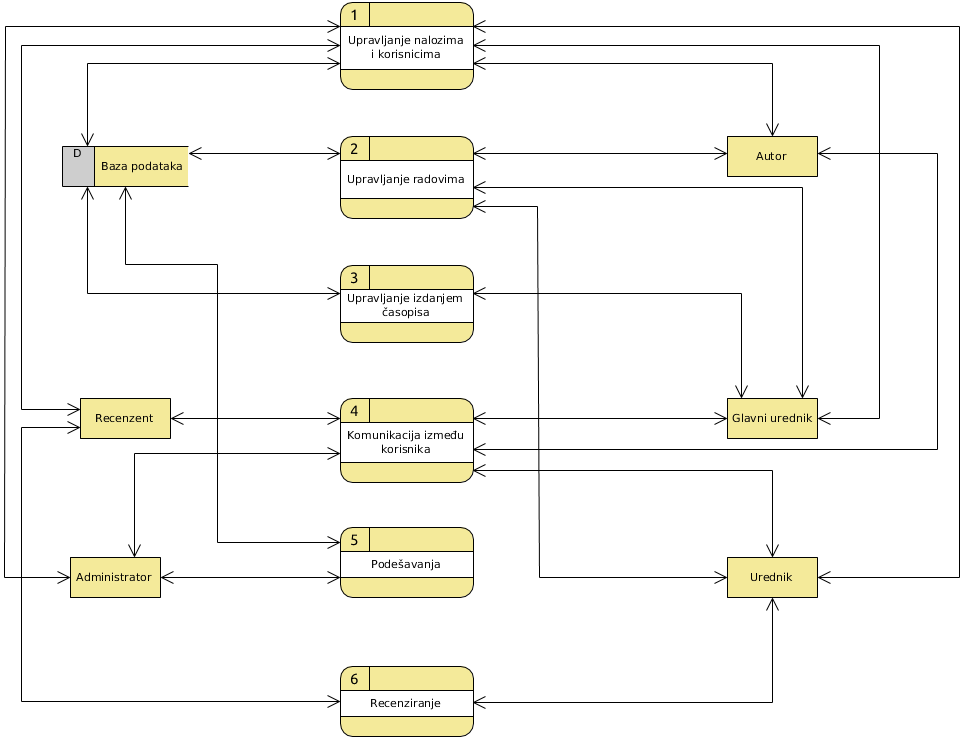
\includegraphics[width=1\linewidth]{Nivo0.jpg}
    \caption{Dijagram toka podataka nivoa 0}
    \label{fig:my_label}
\end{figure}

\section{Slučajevi upotrebe}

\subsection{Upravljanje nalozima i korisnicima}


\begin{figure}[hbt!]
    \centering
    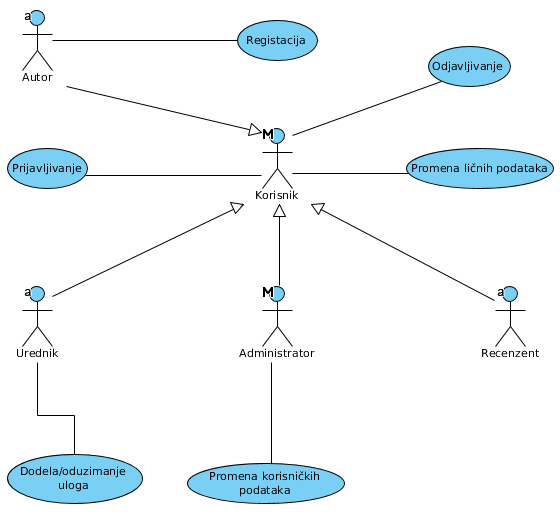
\includegraphics[width=1\linewidth]{UpravljanjeNalozimaIKorisnicima.PNG}
    \caption{Upravljanje nalozima i korisnicima}
    \label{fig:my_label}
\end{figure}

\subsubsection{Registracija korisnika}
\begin{itemize}
    \item Akter: Korisnik
    \item Kratak opis: Korisnik unosi potrebne podatke kako bi se registrovao u sistemu
    \item Preduslov: Korisnik nije već registrovan
    \item Postuslov: Novi korisnik je dodat u sistem
    \item Osnovni tok događaja:
        \begin{enumerate}
            \item Korisnik unosi podatke u formular koji mu se prikazuje nakon zahteva za registracijom %(dok ne uradimo screenshot forme, ovo je placeholder formular sadrzi polja: First Name, Last Name, Title, Email, Confirm email, Password, Repeat Password, URL, Phone, Country, (check option) Available for reviewing role, Google ReCaptcha)
            \item Korisnik pokušava da se registruje
            \item Sistem prikazuje narednu stranicu za potvrdu email adrese
            \item Korisnik potvrđuje svoju email adresu
            \item Sistem uspešno registruje korisnika
        \end{enumerate}
    \item Alternativni tok događaja:
        \begin{enumerate}
            \item Neko od obaveznih polja nije popunjeno
                \begin{enumerate}
                    \item Nakon 2. koraka sistem ispisuje poruku o grešci i zahteva od korisnika da unese podatke koji fale u obaveznim poljima i ta polja bivaju označena.
                    \item Korisnik popunjava tražena polja.
                    \item Korisnik zatim ponavlja korak 2 iz osnovnog toka.
                \end{enumerate}
            \item Vrednosti u poljiva Confirm email i Repeat Password ne odgovaraju vrednostima u poljima Email i Password
                \begin{enumerate}
                    \item Nakon 2. koraka sistem ispisuje poruku o grešci i obaveštava korisnika o nepoklapanju podataka u datim poljima.
                    \item Korisnik ponovo popunjava sporna polja.
                    \item Korisnik zatim ponavlja korak 2 iz osnovnog toka.
                \end{enumerate}
            \item Neko od polja ne odgovara formatu koji je za to polje zadat regularnim izrazom
                \begin{enumerate}
                    \item Nakon 2. koraka sistem ispisuje poruku o grešci i zahteva od korisnika da unese podatke u odgovarajućem formatu za polja koja označava na neki način.
                    \item Korisnik ponovo popunjava tražena polja.
                    \item Korisnik zatim ponavlja korak 2 iz osnovnog toka.
                \end{enumerate}
            \item ReCaptcha ne prepoznaje korisnika kao živu osobu
                \begin{enumerate}
                    \item Nakon 1. koraka sistem ne dozvoljava korisniku da nastavi sa registracijom.
                    \item ReCaptcha se reinicijalizuje.
                    \item Korisnik ponovo pokušava da "reši"\ ReCaptcha.
                    \item Korisnik ponavlja korak c) ovog alternativnog toka 4 dok ne bude moguće preći na korak 2 osnovnog toka.
                    \item Prelazi na korak 2 osnovnog toka.
                \end{enumerate}
        \end{enumerate}
\end{itemize}


\begin{figure}[hbt!]
    \centering
    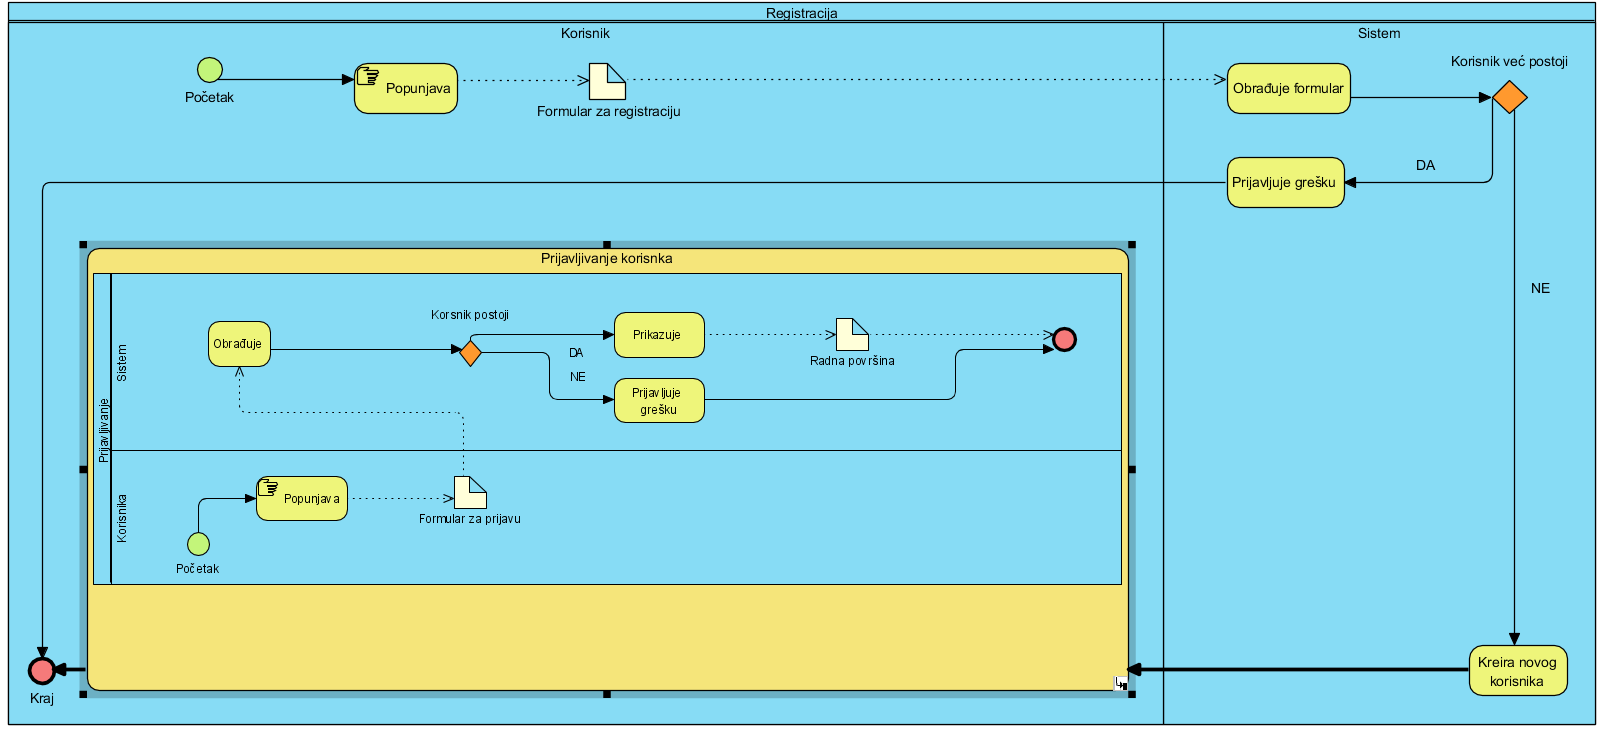
\includegraphics[width=1.2\linewidth]{RegistracijaKorisnika.PNG}
    \caption{Registracija korisnika}
    \label{fig:my_label}
\end{figure}


\subsubsection{Prijavljivanje korisnika}
\begin{itemize}
    \item Akter: Korisnik
    \item Kratak opis: Korisnik unosi potrebne podatke kako bi se ulogovao u sistem
    \item Preduslovi: Korisnik postoji u sistemu
    \item Postuslovi: Nema
    \item Osnovni tok događaja:
        \begin{enumerate}
            \item Korisnik unosi svoju email adresu i šifru u polja koja su za to predoređena
            \item Korisnik šalje sistemu zahtev za prijavu
            \item Sistem autentifikuje korisnika
            \item Sistem prikazuje korisniku početnu stranicu u zavisnosti od uloge:
        %    \begin{enumerate}
         %       \item Administrator - admin panel za upravljanje sistemom
          %      \item Glavni urednik - lista novopristiglih radova
         %       \item Urednik - lista radova koji su poslednji dodeljeni od strane glavnog urednika
          %      \item Recenzent - lista radova koji su poslednji ponuđeni za recenziju od strane urednika
          %      \item Autor - listu svojih radova
          %  \end{enumerate}
        \end{enumerate}
    \item Alternativni tok događaja:
        \begin{enumerate}
            \item Autentifikacija korisnika nije uspela zbog neispravno unetih podataka
                \begin{enumerate}
                    \item Nakon 2. koraka osnovnog toka, sistem ispisuje poruku o neuspešnoj autentikaciji zbog neispravno unetih podataka.
                    \item Korisnik ponavlja korake 1. i 2. osnovnog toka.
                \end{enumerate}
            \item Autentifikacija korisnika nije uspela zbog greške u sistemu
                \begin{enumerate}
                    \item Nakon 2. koraka osnovnog toka, sistem ispisuje poruku o neuspešnoj autentifikaciji zbog greške u sistemu
                    \item Korisnik obaveštava administratora časopisa o postojanju tehničkih problema u sistemu.
                \end{enumerate}
        \end{enumerate}
\end{itemize}



\subsubsection{Dodela/Oduzimanje uloga korisnicima}
\begin{itemize}
    \item Akter: Glavni urednik
    \item Kratak opis: Glavni urednik časopisa dodeljuje/oduzima recenzentsku ili uredničku ulogu postojećem korisniku sistema.
    \item Preduslovi: Postoje korisnici sistema koji nemaju ulogu recenzenta ili urednika. Korisnik kojem glavni urednik želi da dodeli ulogu recenzenta je označio da nema ništa protiv da mu bude dodeljena uloga recenzenta.
    \item Postuslovi: Nema
    \item Osnovni tok događaja:
        \begin{enumerate}
            \item Glavni urednik upućuje upit sistemu za spisak svih korisnika sistema.
            \item Sistem vraća spisak svih korisnika sistema.
            \item Glavni urednik bira korisnika sistema.
            \item Glavni urednik dodeljuje/oduzima ulogu recenzenta ili urednika korisniku sistema.
            \item Sistem čuva izmene o ulozi korisnika.\\
            Ponavljati korake 3, 4 i 5 dok za tim ima potrebe.
        \end{enumerate}
    \item Alternativni tok događaja:
        \begin{enumerate}
            \item Sistem ne vraća uspešno spisak korisnika sistema.
            \begin{enumerate}
                \item U 2. koraku osnovnog toka, sistem ne vraća uspešno spisak korisnika sistema i obaveštava glavnog urednika o grešci.
                \item Glavni urednik se vraća na 1. korak osnovnog toka ili se obraća administratoru.
            \end{enumerate}
            \item Sistem ne čuva izmene o ulozi korisnika.
            \begin{enumerate}
                \item U 5. koraku osnovnog toka, sistem ne čuva izmene o ulozi korisnika i obaveštava glavnog urednika o grešci.
                \item Glavni urednik se vraća na 4. korak osnovnog toka ili se obraća administratoru.
            \end{enumerate}
        \end{enumerate}
\end{itemize}


\begin{figure}[hbt!]
    \centering
    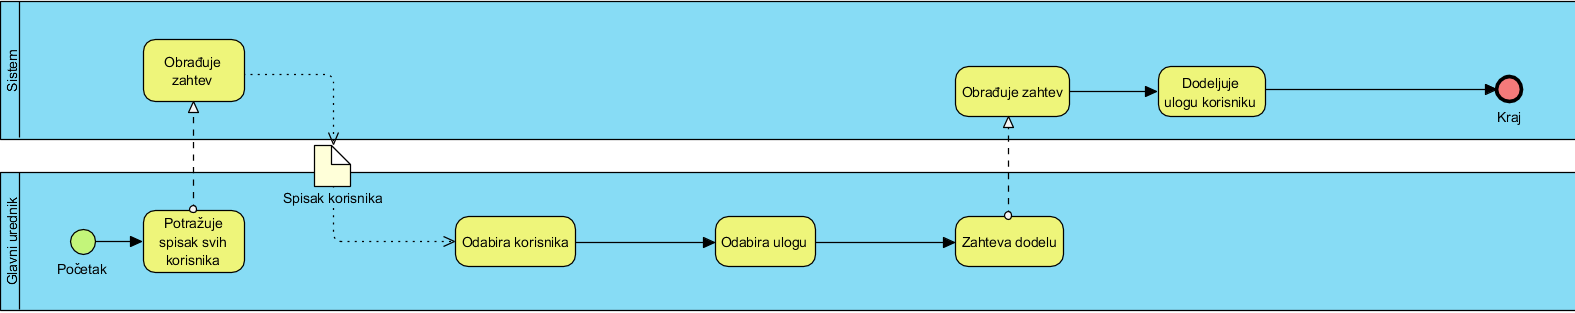
\includegraphics[width=1\linewidth]{DodelaUlogaKorisnicima.PNG}
    \caption{Dodela uloga korisnicima}
    \label{fig:my_label}
\end{figure}



\subsubsection{Promena ličnih podataka}
\begin{itemize}
    \item Akter: Korisnik (Administrator, Glavni urednik, Urednik, Recenzent, Autor)
    \item Kratak opis: Korisnik sistema želi da promeni neke od ličnih podataka
    \item Preduslovi: Korisik postoji u sistemu.
    \item Postuslovi: Nema
    \item Osnovni tok događaja:
        \begin{enumerate}
            \item Korisnik šalje zahtev sistemu za prikaz forme za promenu podataka, koja je slična formi za registraciju, na kojoj korisnik menja željene podatke.
            \item Korisnik menja podatke.
            \item Korisik šalje zahtev sistemu za čuvaje promenjenih podataka.
            \item Sistem je uspešno sačuvao nove podatke.
            \item Sistem obaveštava korisnika o uspešnoj promeni podataka.
        \end{enumerate}
    \item Alternativni tok događaja:
        \begin{enumerate}
            \item Među promenjenim podacima je i email adresa
                \begin{enumerate}
                    \item U 5. koraku osnovnog toka, sistem obaveštava korisnika o uspešnosti promene svih korisničkih podataka osim email adrese.
                    \item Sistem ispisuje obaveštenje korisniku da treba da potvrdi svoju novu email adresu tako što će posetiti link koji mu je na tu adresu poslat.
                    \item Korisnik šalje sistemu potvrdu nove email adrese
                    \item Sistem obaveštava korisika o uspešnoj promeni email adrese.
                \end{enumerate}
            \item Neko od obaveznih polja nije popunjeno ili neko od polja ne odgovara formatu koji je za to polje zadat regularnim izrazom
                \begin{enumerate}
                    \item U 4. koraku osnovnog toka, sistem ispisuje poruku o grešci i obaveštava korisnika da podaci nisu uspešno izmenjeni.
                    \item Korisnik se vraća na korak 1. osnovnog toka.
                \end{enumerate}
        \end{enumerate}
\end{itemize}


\begin{figure}[hbt!]
    \centering
    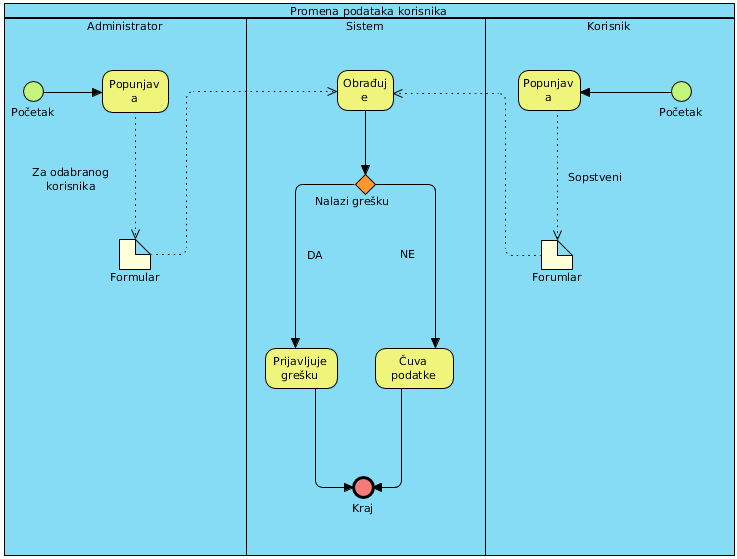
\includegraphics[width=1\linewidth]{PromenaPodatakaKorisnika.PNG}
    \caption{Promena podataka korisnika}
    \label{fig:my_label}
\end{figure}


\subsubsection{Promena korisničkih podataka}
\begin{itemize}
    \item Akter: Administrator
    \item Kratak opis: Administrator sistema želi da promeni neke od ličnih podataka drugih korinika
    \item Preduslovi: Nema
    \item Postuslovi: Nema
    \item Osnovni tok događaja:
        \begin{enumerate}
            \item Administrator šalje sistemu zahtev za prikaz spiska korisnika kojima može menjati lične informacije.
            \item Sistem prikazuje administratoru sistema spisak korisika.
            \item Administrator bira željenog korisnika.
            \item Sistem prikazuje administrator formular na kome može menjati lične podatke korisnika (sve osim email-a).
            \item Administrator menja lične podatke koristika.
            \item Administrator šalje sistemu zahtev za čuvanje novih ličnih podataka korisnika.
            \item Sistem je uspešno promenio podatke odaranog korisnika.
            \item Sistem obaveštava administratora o uspešnoj akciji.
        \end{enumerate}
    \item Alternativni tok događaja:
        \begin{enumerate}
            \item Neko od obaveznih polja nije popunjeno ili neko od polja ne odgovara formatu koji je za to polje zadat regularnim izrazom
                \begin{enumerate}
                    \item U 7. koraku osnovnog toka sistem ispisuje poruku o grešci i obaveštava administratora da podaci nisu uspešno izmenjeni.
                    \item Administrator se vraća na 5. korak osnovnog toka.
                \end{enumerate}
        \end{enumerate}
\end{itemize}

\subsection{Upravljanje izdanjem časopisa}

\subsubsection{Odabir prihvaćenih radova za tekuće izdanje časopisa}
\begin{itemize}
    \item Akter: Glavni urednik časopisa
    \item Kratak opis: Glavni urednik časopisa razmatra sve radove koji su prihvaćeni i vrši odabir radova koji će ući u tekuće izdanje časopisa.
    \item Preduslovi: Postoje prihvaćeni radovi koji nisu objavljeni
    \item Postuslovi: Nema
    \item Osnovni tok događaja:
        \begin{enumerate}
            \item Glavni urednik upućuje upit sistemu za sve prihvaćene radove koji nisu objavljeni ni u jednom dosadašnjem izdanju časopisa.
            \item Sistem vraća spisak svih takvih radova.
            \item Glavni urednik pregleda sledeći rad.
            \item Glavni urednik donosi odluku da li će rad ući u tekuće izdanje časopisa.
            \item Ukoliko će rad ući u tekuće izdanje: Glavni urednik šalje zahtev sistemu da se rad ubaci u radnu verziju tekućeg izdanja časopisa.
            \item Sistem dodaje rad u radnu verziju tekućeg izdanja.\\ Ponavljati korake 3, 4, 5 i 6 dok se postigne traženi broj radova ili traženi broj stranica za tekuće izdanje)
        \end{enumerate}
    \item Alternativni tok događaja:
        \begin{enumerate}
            \item Sistem ne vraća uspešno spisak prihvaćenih radova.
                \begin{enumerate}
                    \item U 2. koraku osnovnog toka, sistem ne vraća uspešno spisak prihvaćenih radova i obaveštava glavnog urednika o grešci.
                    \item Glavni urednik se vraća na 1. korak osnovnog toka ili se obraća se administratoru.
                \end{enumerate}
            \item Sistem ne otvara uspešno sledeći rad koji glavni urednik želi da pregleda.
                \begin{enumerate}
                    \item U 3. koraku osnovnog toka, sistem ne otvara uspešno rad koji glavni urednik želi da pregleda i prikazuje obaveštenje o grešci.
                    \item Glavni urednik se vraća na 3. korak osnovnog toka ili se obraća administratoru časopisa.
                \end{enumerate}
            \item Sistem ne dodaje rad u radnu verziju tekućeg izdanja.
            \begin{enumerate}
                \item Sistem ne dodaje rad u radnu verziju tekučeg izdanja i prikazuje poruku o grešci.
                \item Glavni urednik se vraća na 6. korak osnovnog toka ili se obraća administratoru.
            \end{enumerate}
        \end{enumerate}
\end{itemize}

\begin{figure}[hbt!]
    \centering
    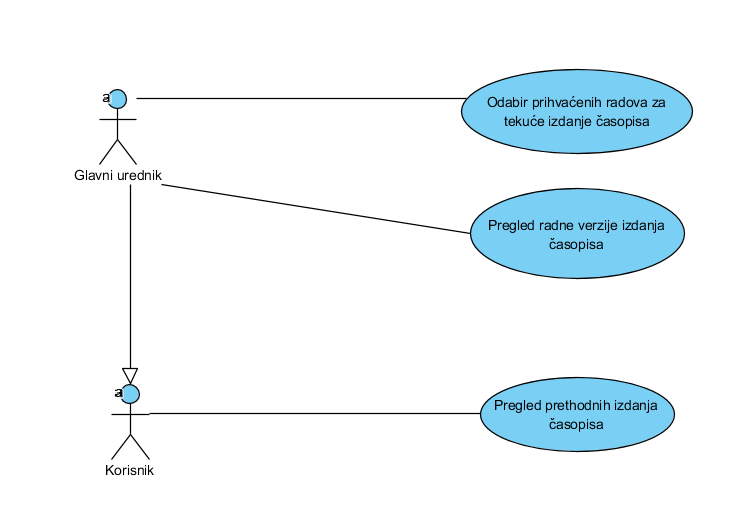
\includegraphics[width=\linewidth]{UpravljanjeIzdanjemCasopisa.PNG}
    \caption{Upravljanje izdanjem časopisa}
    \label{fig:my_label}
\end{figure}

\subsubsection{Pregled radne verzije izdanja časopisa}
\begin{itemize}
    \item Akter: Glavni urednik
    \item Kratak opis: Glavni urednik vrši pregled radne verzije tekućeg izdanja časopisa.
    \item Preduslovi: Nema
    \item Postuslovi: Nema
    \item Osnovni tok događaja:
        \begin{enumerate}
            \item Glavni urednik zahteva od sistema pregled radne verzije tekućeg izdanja časopisa.
            \item Sistem prikazuje radnu verziju tekućeg izdanja časopisa.
        \end{enumerate}
    \item Alternativni tok događaja:
        \begin{enumerate}
            \item Sistem ne prikazuje radnu verziju časopisa.
            \begin{enumerate}
                \item U 2. koraku osnovnog roka, sistem ne prikazuje radnu verziju časopisa i obaveštava glavnog urednika o grešci.
                \item Glavni urednik se vraća na 1. korak osnovnog toka ili se obraća administratoru.
            \end{enumerate}
        \end{enumerate}
\end{itemize}

\subsubsection{Pregled prethodnih izdanja časopisa}
\begin{itemize}
    \item Akter: Korisnik
    \item Kratak opis: Korisnik informacionog sistema vrši pregled prethodnog izdanja časopisa.
    \item Preduslovi: Postoji bar jedno izdanje časopisa.
    \item Postuslovi: Nema
    \item Osnovni tok događaja:
        \begin{enumerate}
            \item Korisnik zahteva od sistema pregled spisak prethodnih izdanja časopisa.
            \item Sistem prikazuje spisak prethodnih izdanja.
            \item Korisnik bira izdanje koje želi da pregleda.
            \item Sistem mu prikazuje traženo izdanje časopisa.
        \end{enumerate}
    \item Alternativni tok događaja:
        \begin{enumerate}
            \item Sistem ne prikazuje spisak prethodnih izdanja.
            \begin{enumerate}
                \item Sistem ne prikazuje spisak prethodnih izdanja časopisa i obaveštava korisnika o grešci.
                \item Korisnik se vraća na 1. korak osnovnog toka, odustaje ili se obraća administratoru.
            \end{enumerate}
            \item Sistem ne prikazuje traženo izdanje časopisa.
            \begin{enumerate}
                \item Sistem ne prikazuje traženo izdanje časopisa i obaveštava korisnika o grešci.
                \item Korisnik se vraća na 3. korak osnovnog toka, pri čemu eventualno menja izdanje koje želi da pregleda, ili se obraća administratoru.
            \end{enumerate}
        \end{enumerate}
\end{itemize}

\subsection{Upravljanje časopisom}

\subsubsection{Promena podataka časopisa}

\begin{figure}[hbt!]
    \centering
    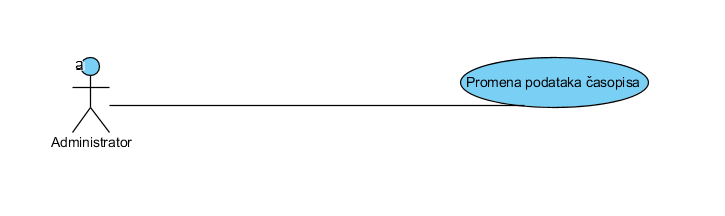
\includegraphics[width=\linewidth]{PromenaPodatakaCasopisa.png}
    \caption{Promena podataka časopisa}
    \label{fig:my_label}
\end{figure}

\begin{itemize}
    \item Akter: Administrator sistema
    \item Kratak opis: Administrator menja podatke časopisa
    \item Preduslov: nema
    \item Postuslov: nema
    \item Osnovni tok događaja:
        \begin{enumerate}
            \item Administrator pristupa obrascu za menjanje podataka
            \item Administrator unosi podatke u formu
            \item Adminstrator šalje zahtev za čuvanjem novih podataka
            \item Sistem je sačuvao nove podatke
            \item Sistem obaveštava koriniska o sačuvanim izmenama
        \end{enumerate}
    \item Alternativni tok događaja:
        \begin{enumerate}
            \item Koraka 4. osnovnog toka: Sistem ne može da sačuva nove podatke
                \begin{enumerate}
                    \item Administrator popravlja unete podatke tako da budu u saglasnosti sa bazom podataka
                    \begin{enumerate}
                        \item Administrator šalje zahtev za čuvanjem podataka
                        \item Ako je sistem sačuvao nove podatke, prelazi se na korak 5. osnovnog toka.
                        \item Ako ne, prelazi se na korak 1.b) alternativnog toka.
                    \end{enumerate}
                    \item Administrator proverava internet konekciju i uspešno je podešava.
                    \begin{enumerate}
                        \item Ponovo šalje zahtev za čuvanjem podataka
                        \item Ako je sistem sačuvao nove podatke, prelazi se na korak 5. osnovnog toka.
                        \item Ako ne, prelazi se na korak 1.c) alternativnog toka.
                    \end{enumerate}
                    \item Administrator proverava da li je funkcionalnost slanja podataka preko forme dobro implementirana.
                    \begin{enumerate}
                        \item Administrator popravlja funkcionalnost i pokušava ponovo da sačuva podatke.
                        \item Administrator šalje zahtev za čuvanjem podataka
                        \item Ako je sistem sačuvao nove podatke, prelazi se na korak 5. osnovnog toka.
                        \item Ako ne, prelazi se na korak 1.d) alternativnog toka.
                    \end{enumerate}
                    \item Ozbiljna greška sistema. Administrator traži grešku i pokušava da je otkloni.
                \end{enumerate}
        \end{enumerate}
\end{itemize}

\begin{figure}[hbt!]
    \centering
    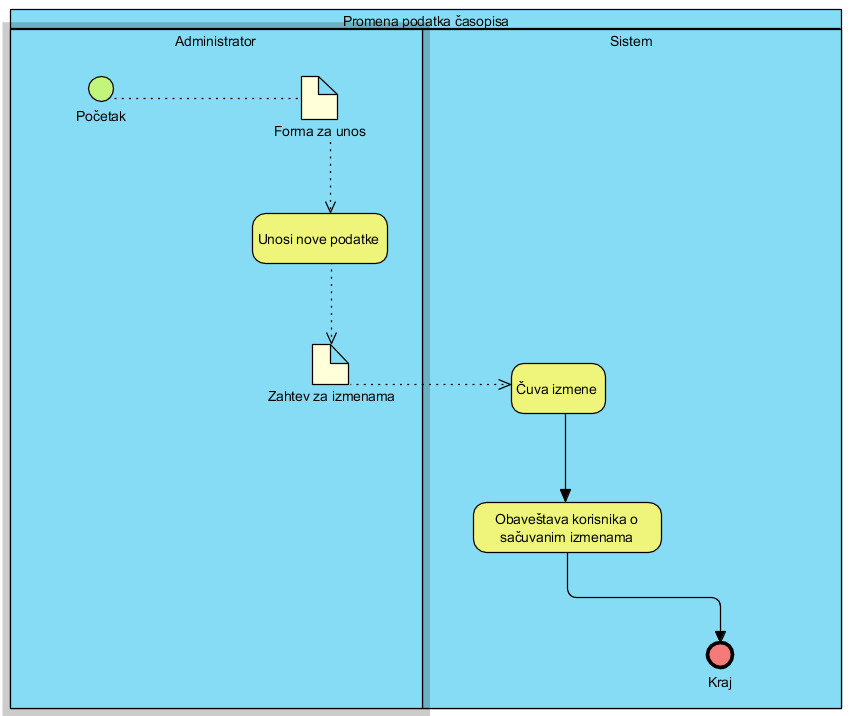
\includegraphics[width=\linewidth]{PromenaPodatakaCasopisa.PNG}
    \caption{Promena podataka časopisa}
    \label{fig:my_label}
\end{figure}

\subsection{Upravljanje radovima}

\begin{figure}[hbt!]
    \centering
    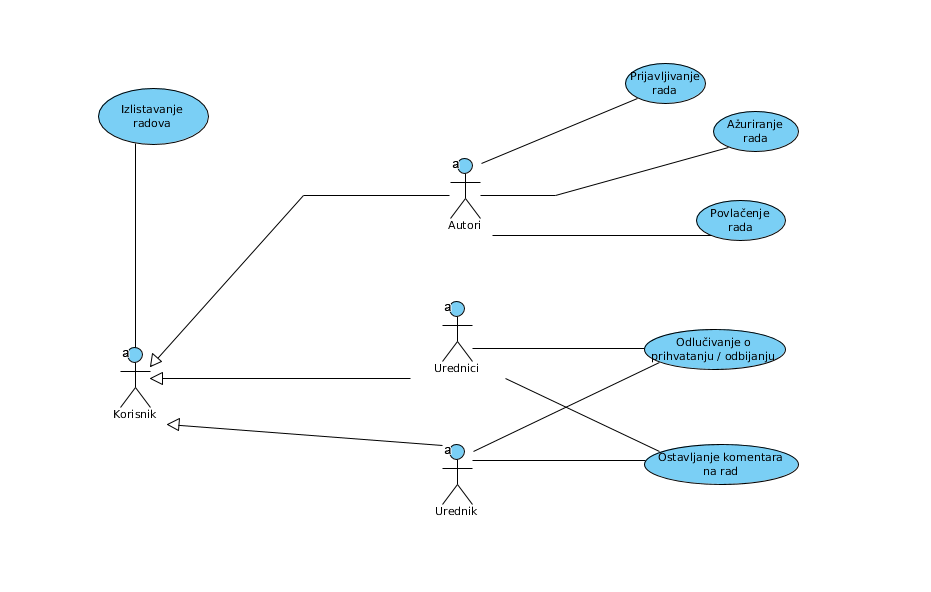
\includegraphics[width=1\linewidth]{UpravljanjeRadovima.png}
    \caption{Upravljanje radovima}
    \label{fig:my_label}
\end{figure}


\begin{figure}[hbt!]
    \center
    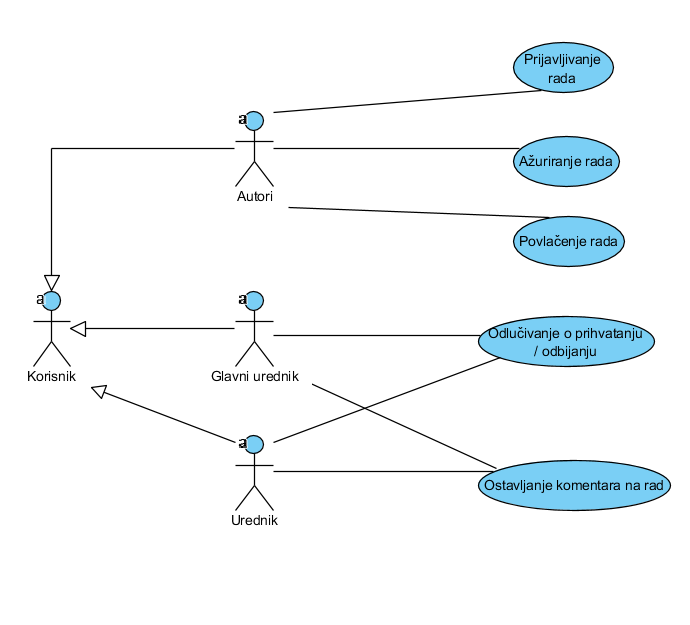
\includegraphics[width=1\linewidth]{UpravljanjeRadovima.jpg}
    \caption{Dijagram toka podataka nivoa 1 Upravljanje radovima}
    \label{fig:my_label}
\end{figure}

\subsubsection{Izlistavanje radova}
\begin{itemize}
    \item Akter: Korisnik
    \item Kratak opis: Korisnik izlistava radove po zadatom uslovu u filteru.
    \item Preduslovi: Korisnik je registrovan u sistemu.
    \item Postuslovi: Nema
    \item Osnovni tok događaja:
        \begin{enumerate}
            \item Korisnik bira kriterijum u filteru.
            \item Korisnik šalje zahtev sistemu za prikazivanje svih radova koji zadovoljavaju zadati kriterijum.
            \item Sistem šalje podatke o radovima i islistava ih.
        \end{enumerate}
    \item Alternativni tok događaja:
        \begin{enumerate}
            \item Korak 2. osnovnog toka: Sistem ne nalazi podatke ni o jednom radu.
            \begin{enumerate}
                \item Sistem obaveštava korisnika o nepostojanju radova sa zadatim kriterijumom.
                \item Korisnik se vraća na 1. korak osnovnog toka ili odustaje.
            \end{enumerate}
        \end{enumerate}
\end{itemize}

\begin{comment}
\subsubsection{Recenzent izlistava radove koje recenzira}
\begin{itemize}
    \item Akter: Recenzent
    \item Kratak opis: Recenzent izlistava radove na koje je prihvatio da recenzira.
    \item Preduslovi: Recenzent je korisnik sistema sa ulogom Recenzent.
    \item Postuslovi: Nema
    \item Osnovni tok događaja:
        \begin{enumerate}
            \item Recenzent šalje zahtev sistemu za prikazivanje svih radova koje je prihvatio da recenzira.
            \item Sistem šalje podatke o radovima i islistava ih.
        \end{enumerate}
    \item Alternativni tok događaja:
        \begin{enumerate}
            \item Korak 2. osnovnog toka: Sistem ne nalazi podatke ni o jednom radu.
            \begin{enumerate}
                \item Sistem obaveštava korisnika o nepostojanju radova na kojima je prihvatio recenzentsku ulogu.
                \item Recenzent se vraća na 1. korak osnovnog toka ili odustaje.
            \end{enumerate}
        \end{enumerate}
\end{itemize}

\subsubsection{Urednik izlistava radove}
\begin{itemize}
    \item Akter: Urednik
    \item Kratak opis: Urednik izlistava radove koje je dobio od glavnog uredinka.
    \item Preduslovi: Recenzent je korisnik sistema sa ulogom Recenzent.
    \item Postuslovi: Nema
    \item Osnovni tok događaja:
        \begin{enumerate}
            \item Recenzent šalje zahtev sistemu za prikazivanje svih radova koje je prihvatio da recenzira.
            \item Sistem šalje podatke o radovima i islistava ih.
        \end{enumerate}
    \item Alternativni tok događaja:
        \begin{enumerate}
            \item Korak 2. osnovnog toka: Sistem ne nalazi podatke ni o jednom radu.
            \begin{enumerate}
                \item Sistem obaveštava korisnika o nepostojanju radova na kojima je prihvatio recenzentsku ulogu.
                \item Recenzent se vraća na 1. korak osnovnog toka ili odustaje.
            \end{enumerate}
        \end{enumerate}
\end{itemize}
\end{comment}



\subsubsection{Prijavlivanje rada}

\begin{itemize}
    \item Akter: Autor
    \item Kratak opis: Autor prijavljuje rad.
    \item Preduslovi: Autor je korisnik sistema sa ulogom Autor.
    \item Postuslovi: Rad se nalazi u sistemu.
    \item Osnovni tok događaja:
        \begin{enumerate}
            \item Autor unosi potrebne podatke podatke za rad.
            \item Autor šalje zahtev za prijavljivanje rada.
            \item Sistem čuva rad.
            \item Sistem obaveštava autora o uspešnom prijavljivanju rada.
        \end{enumerate}
    \item Alternativni tok događaja:
        \begin{enumerate}
            \item Korak 3. osnovnog toka: Sistem nije uspeo da sačuva rad.
            \begin{enumerate}
                \item Sistem obaveštava korisnika o grešci.
                \item Autor se vraća na 1. korak osnovnog toka ili odustaje.
            \end{enumerate}
        \end{enumerate}
\end{itemize}

\subsubsection{Ažuriranje rada}
\begin{itemize}
    \item Akter: Autor
    \item Kratak opis: Autor, nakon dorade, prijavljuje novu verziju rada
    \item Preduslovi: Rad je prijavljen
    \item Postuslovi: Nova verzija rada je sačuvana
    \item Osnovni tok događaja:
        \begin{enumerate}
           \item Autor popunjava formular za prijavu nove verzije rada.
           \item Autor šalje zahtev za čuvanjem nove verzije rada.
           \item Sistem je sačuvao novu verziju rada.
           \item Sistem obaveštava autora o sačuvanoj novoj verziji rada.
        \end{enumerate}
    \item Alternativni tok događaja:
        \begin{enumerate}
            \item Korak 3. osnovnog toka: Sistem nije uspeo da sačuva novu verziju rada.
            \begin{enumerate}
                \item Sistem obaveštava korisnika o grešci.
                \item Autor se vraća na 1. korak osnovnog toka ili odustaje.
            \end{enumerate}
        \end{enumerate}
\end{itemize}

\subsubsection{Povlačenje rada}
\begin{itemize}
    \item Akter: Autor
    \item Kratak opis: Autor povlači rad iz časopisa
    \item Preduslovi: Rad je prijavljen
    \item Postuslovi: Nema
    \item Osnovni tok događaja:
        \begin{enumerate}
           \item Autor popunjava formular za povlačenjem rada.
           \item Autor šalje zahtev za povlačenjem rada.
           \item Sistem je označio rad kao povučen, ali ga nije izbrisao iz baze podataka.
           \item Sistem obaveštava autora da je rad povučen.
        \end{enumerate}
    \item Alternativni tok događaja: nema
\end{itemize}

\subsubsection{Odlučivanje o prihvatanju/odbijanju rada}
\begin{itemize}
    \item Akter: Glavni urednik, Urednik
    \item Kratak opis: (Glavni) Urednik menja prihvata ili odbija rad. Glavni urednik može promeniti ovaj status već prihvaćenom/odbijenom radu.
    \item Preduslovi: Rad se nalazi u sistemu. Uredniku je rad prosledjen od strane glavnog urednika. Uradnik i Glavni urednik su registrovani u sistemu
    \item Postuslovi: Rad ima novo stanje u sistemu.
    \item Osnovni tok događaja:
        \begin{enumerate}
            \item (Glavni) Urednik odabira rad.
            \item (Glavni) Urednik bira da li je rad odbijen ili prihvaćen.
            \item (Glavni) Urednik šalje sistemu zahtev za čuvanjem novog statusa rada.
            \item Sistem je sačuvao novi status rada.
            \item Sistem obaveštava (glavnog) urednika o uspešnom prihvatanju/odbijanju rada.
        \end{enumerate}
    \item Alternativni tok događaja:
        \begin{enumerate}
            \item Korak 2. osnovnog toka: Rad prethodno nije recenziran.
                \begin{enumerate}
                    \item (Glavnom) Uredniku se prikazuje polje u kom ostavlja komentar na rad.
                    \item (Glavni) Urednik se vraća na 3. korak osnovnog toka ili odustaje.
                \end{enumerate}
            \item Korak 4. osnovnog toka: Sistem nije uspeo da sačuva rad.
            \begin{enumerate}
                \item Sistem obaveštava (glavnog) urednika o grešci.
                \item (Glavni) Urednik se vraća na 1. korak osnovnog toka ili odustaje.
            \end{enumerate}
        \end{enumerate}
\end{itemize}

\subsubsection{Ostavljanje komentara na rada}
\begin{itemize}
    \item Akter: Glavni urednik i urednik
    \item Kratak opis: Glavni urednik i urednik ostavljaju komentar na rad
    \item Preduslovi: Rad je prijavljen
    \item Postuslovi: Komentar je sačuvan
    \item Osnovni tok događaja:
        \begin{enumerate}
           \item (Glavni) urednik bira rad na koji želi da ostavi komentar.
           \item (Glavni) urednik piše tekst komentara.
           \item (Glavni) urednik šalje zahtev za čuvanjem komentara.
           \item Sistem je sačuvao komentar.
           \item Sistem šalje poruku sa odgovarajućim šablonom autoru koji je prijavio rad.
           \item Sistem obaveštava (glavnog) urednika o ostavljanju komentara na rad.
        \end{enumerate}
    \item Alternativni tok događaja:
        \begin{enumerate}
            \item Koraka 2. osnovnog toka: (Glavni) urednik nije ukucao nikakav tekst
            \begin{enumerate}
                \item Sistem ignoriše zahtev.
                \item Sistem obaveštava (glavnog) urednika o tome da nije uneo tekst.
                \item Tok se nastavlja na koraku 1 glavnog toka.
            \end{enumerate}
            \item Korak 5. osnovnog toka: Sistem nije uspeo da pošalje poruku autoru.
            \begin{enumerate}
                \item Sistem obaveštava (glavnog) urednika da nije poslao poruku autoru o novom komentaru na rad.
                \item Sistem obaveštava (glavnog) urednika da je potrebno da sam obavesti autora o novom komentaru.
                \item Tok se nastavlja na koraku 6 glavnog toka.
            \end{enumerate}
        \end{enumerate}
\end{itemize}

\subsection{Recenziranje}

\begin{figure}[hbt!]
    \centering
    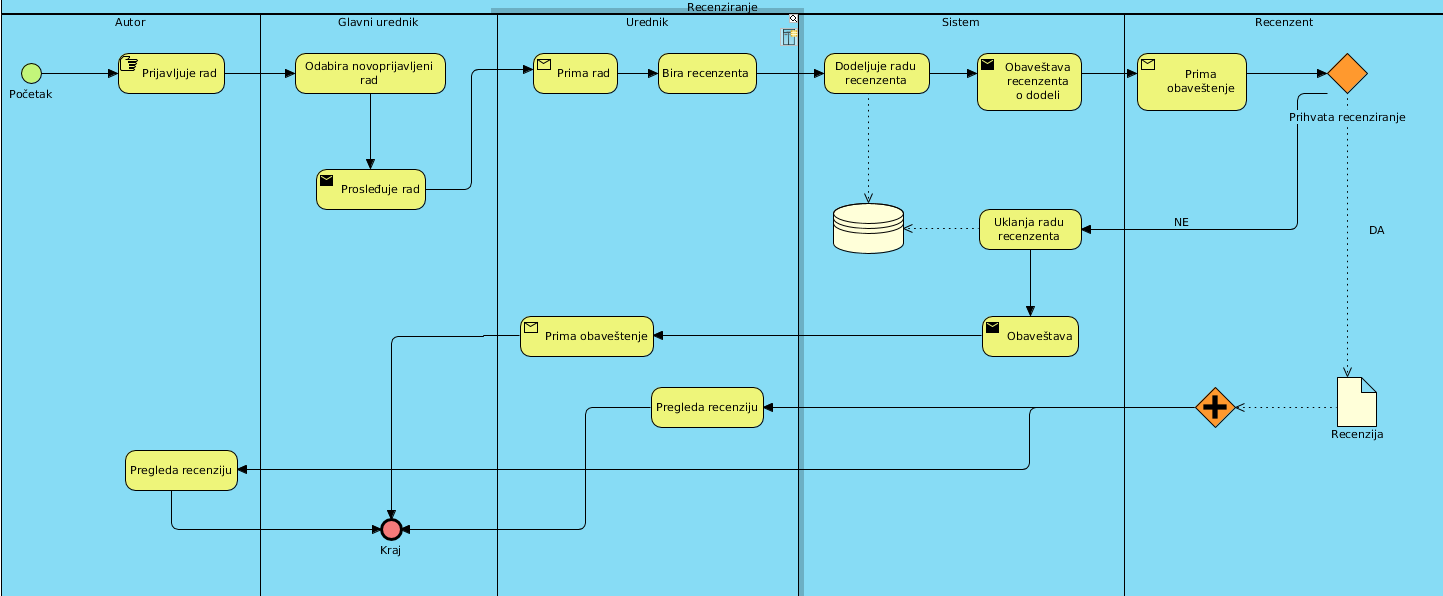
\includegraphics[width=1.3\linewidth]{Recenziranje.PNG}
    \caption{Recenziranje}
    \label{fig:my_label}
\end{figure}

\subsubsection{Odabir recenzenta}
\begin{itemize}
    \item Akter: Urednik
    \item Kratak opis: Urednik bira recenzente za prijavljeni rad
    \item Preduslovi: Radu nisu dodeljeni recenzenti
    \item Postuslovi: Nema
    \item Osnovni tok događaja:
        \begin{enumerate}
           \item Urednik šalje sistemu zahtev za dobijanje spiska recenzenata.
           \item Sistem prikazuje spisak recenzenata.
           \item Urednik bira recenzenta.
           \item Urednik šalje recenzentu ponudu za recenziranje rada.
           \item Sistem šalje mejl recenzentu sa ponudom za recenziranje.
           \item Sistem obaveštava urednika o uspešno poslatom mejlu.
        \end{enumerate}
    \item Alternativni tok događaja:
        \begin{enumerate}
            \item Sistem ne prikazuje spisak recenzenata zbog greške.
            \begin{enumerate}
                \item U 2. koraku osnovnog toka, sistem ne prikazuje spisak recenzenata i prikazuje poruku o grešci.
                \item Urednik se vraća na 1. korak osnovnog toka ili se obraća administratoru.
            \end{enumerate}
            \item Nema recenzenata u sistemu.
            \begin{enumerate}
                \item U 2. koraku osnovnog toka, sistem prikazuje prazan spisak recenzenata.
                \item Urednik se obraća glavnom uredniku.
            \end{enumerate}
            \item Sistem nije uspešno poslao mejl recenzentu.
            \begin{enumerate}
                \item U 5. koraku osnovnog toka, sistem nije uspešno poslao mejl recenzentu,
                \item Urednik se vraća na 4. korak osnovnog toka ili se obraća administratoru.
            \end{enumerate}
        \end{enumerate}
\end{itemize}

\begin{figure}[hbt!]
    \centering
    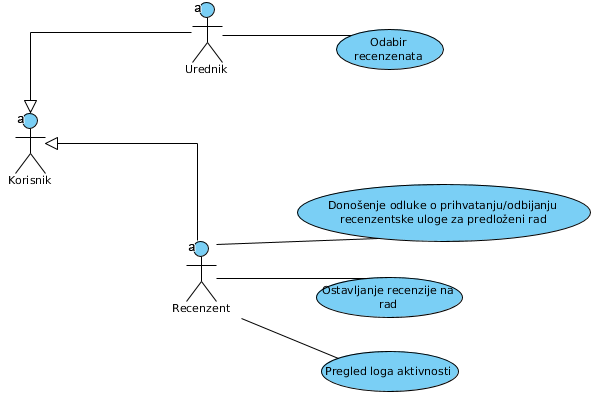
\includegraphics[width=\linewidth]{RecenziranjeUseCase.PNG}
    \caption{Dijagram slučaja upotrebe Recenziranje}
    \label{fig:my_label}
\end{figure}

\subsubsection{Donošenje odluke o prihvatanju/odbijanju recenzentske uloge}
\begin{itemize}
    \item Akter: Recenzent
    \item Kratak opis: Recenzent donosi odluku da li prihvata ili odbija recenzentsku ulogu za prijavljeni rad.
    \item Preduslovi: Recenzent je dobio ponudu da recenzira rad.
    \item Postuslovi: Nema
    \item Osnovni tok događaja:
        \begin{enumerate}
            %\item Recenzent donosi odluku da li prihvata da recenzira rad.
            %\item Recenzent prihvata da recenzira rad.
            %    \begin{enumerate}
            %        \item Slučaj upotrebe se završava.
            %    \end{enumerate}
            \item Recenzent odbija da recenzira rad.
                \begin{enumerate}
                    \item Recenzent šalje zahtev sistemu za uklanjanje sa spiska recenzenata za taj rad.
                    \item Sistem otvara formular za pisanje mejla uredniku.
                    \item Recenzent šalje odgovor uredniku.
                    \item Sistem šalje mejl uredniku.
                    \item Sistem uklanja recenzenta sa spiska.
                    \item Sistem obaveštava recenzenta o uspešnom uklanjanju sa spiska.
                \end{enumerate}
        \end{enumerate}
    \item Alternativni tok događaja:
        \begin{enumerate}
            \item Sistem ne šalje mejl uredniku.
            \begin{enumerate}
                \item U koraku (d) osnovnog toka sistem ne uklanja uspešno recenzenta sa spiska recenzenata za taj rad.
                \item Sistem obaveštava recenzenta o grešci.
                \item Recenzent se vraća na korak (d) osnovnog toka ili se obraća administratoru.
            \end{enumerate}
            \item Sistem ne uklanja recenzenta sa spiska.
            \begin{enumerate}
                \item U koraku (e) osnovnog toka sistem ne uklanja uspešno recenzenta sa spiska recenzenata za taj rad.
                \item Sistem obaveštava recenzenta o grešci.
                \item Recenzent se vraća na korak (a) osnovnog toka ili se obraća administratoru.
            \end{enumerate}
        \end{enumerate}
\end{itemize}

\subsubsection{Ostavljanje recenzije na rad}
\begin{itemize}
    \item Akter: Recenzent
    \item Kratak opis: Recenzent ostavlja svoju recenziju na rad u sistemu.
    \item Preduslov: Recenzent je dodeljen datom radu.
    \item Postuslov: Nema
    \item Osnovni tok događaja:
        \begin{enumerate}
            \item Recenzent popunjava polja formulara za recenziju.
            \item Recenzent šalje zahtev sistemu za objavljivanje recenzije.
            \item Sistem čuva podatke o receziji.
            \item Sistem obaveštava recenzenta o uspešno sačuvanoj recenziji.
        \end{enumerate}
    \item Alternativni tokovi:
        \begin{enumerate}
            \item Sistem ne čuva podatke o recenziji.
            \begin{enumerate}
                \item U 3. koraku osnovnog toka sistem ne čuva uspešno podatke o recenziji.
                \item Sistem obaveštava recenzenta o grešci.
                \item Recenzent se vraća na 2. korak osnovnog toka ili se obraća administratoru.
            \end{enumerate}
        \end{enumerate}
\end{itemize}

\subsubsection{Pregled loga aktivnosti}
\begin{itemize}
    \item Akter: Recenzent
    \item Kratak opis: Recenzent pregleda spisak svih radova koje je prihvatio ili odbio da recenzira
    \item Preduslov: Recenzent poseduje spisak aktivnosti
    \item Postuslov: Nema
    \item Osnovni tok događaja:
        \begin{enumerate}
            \item Recenzent zahteva spisak svojih aktivnosti
            \item Sistem ispisuje spisak aktivnosti
        \end{enumerate}
\end{itemize}

\subsection{Komunikacija među korisnicima}

\subsubsection{Zahtev za slanje poruke (emaila)}
\begin{itemize}
    \item Akter: Korisnik
    \item Kratak opis: Korisnik šalje email koristeći usluge sistema
    \item Preduslovi: Korisnik je registrovan u sistemu.
    \item Postuslovi: Nema
    \item Osnovni tok događaja:
        \begin{enumerate}
            \item Korisnik zahteva spisak postojećih šablona.
            \item Sistem prikazuje korisniku spisak šablona.
            \item Korisnik bira željeni šablon.
            \item Sistem prikazuje sadržaj šablona.
            \item Korisnik označava da želi da nastavi sa slanjem šablona.
            \item Sistem prikazuje imena korisnika sistema.
            \item Korisnik bira korisnike sa liste.
            \item Korisnik šalje zahtev za slanjem poruke.
            \item Sistem šalje email na adresu korisnika.
            \item Sistem obaveštava korisnika o uspešno poslatoj poruci.
        \end{enumerate}
    \item Alternativni tok događaja:
        \begin{enumerate}
            \item Korak 5. osnovnog toka: Korisnik želi da izmeni šablon.
            \begin{enumerate}
                \item Korisnik vrši potrebne izmene u tekstu ili izmenu šablona.
                \item Ako korisnik ne želi da se novi šablon sačuva u bazi prelazi na korak 5 glavnog toka.
                \item Korisnik šalje sistemu zahtev za čuvanjem novog šablona.
                \item Sistem čuva šablon.
                \item Sistem obaveštava korisnika o čuvanju šablona.
                \item Korisnik se vraća na 5. korak osnovnog toka.
            \end{enumerate}
        \end{enumerate}
\end{itemize}

\begin{figure}[hbt!]
    \centering
    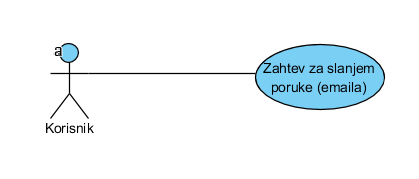
\includegraphics[width=0.8\linewidth]{KomunikacijaIzmedjuKorisnika.PNG}
    \caption{Zahtev za slanjem poruke (emaila)}
    \label{fig:my_label}
\end{figure}

\subsection{Model baze podataka}

Za Korisnika se prati id, ime, prezime, email, sifra, telefon, adresa, postanski broj, vreme poslednjeg logina. Korisnik Upravlja svojim sopstvenim podešavanjima - može upravljati samo svojim podacima, ali i ne mora. Način komunikacije između dva korisnika se ostvaruje tako što korisnik drugom korisniku Šalje šablon za koji se prati id i tekst šablona - korisnik može slati više šablona, ali ne mora slati ni jedan. Šablon može biti poslat od strane više korisnika, ali ne mora ni jedan.

Korisnik Ima ulogu u sistemu, i za tu Ulogu se prati id i naziv. Mora imati jednu ulogu, ali može i više, a ulogu mora imati bar jedan korisnik, ali može i više. Uloge mogu biti: glavni urednik, urednik, autor, recenzent, administrator. Prilikom priljavljivanja na sistem svi korisnici su autori (sem administratora), a glavni urednik (i samo on) im kasnije Dodeljuje uloge, a on sam može dodeliti više uloga. Uloga Obezbeđuje dodatne Privilegije korisnicima sistema, za koje se prati id i naziv. Uloga obezbeđuje barem jednu, a može i više privilegija, privilegije moraju biti dodeljene barem jednoj ulazi, ali mogu i više.

Administrator može da Menja podatke- ostalih korisnika, kao i da Menja podešavanja samog časopisa. Podešavanja samo jednog časopisa menja samo administrator, koji jedini može menjati podatke ostalih korisnika i to više njih, ali ni ne mora.

Autor Prijavljuje Rad, za koji se prati id, naslov, link ka pdf verziji, status, da li je objavljen. On može prijaviti više radova, a ne mora ni jedan, ali samo jedan autor može prijaviti rad. Samo onaj ko je prijavio rad može i da ga povuče, a onaj ko je prijavio radove može da povuče i više svojih radova, ali ne mora ni jedan.

Rad može imati jednu ili više Verzija, a sama verzija može biti verzija samo jednog rada.

Recenzent Objavljuje Recenziju za koju se prati id, komentar, rad na koji je ostavljena, koji recenzent je objavio i za tu objavu se čuvaju vreme i datum. Recenzent može objaviti više recenzija, ali ne mora ni jednu, a recenziju mora objaviti barem jedan recenzent, ali može i više.

(Glavni) urednik može a ne mora da Ostavlja komentar na rad, i to na njih više, a rad može komentarisati i njih više, ali ne mora niko.

Glavni urednik i samo on može da Uređuje Izdanje časopisa za koje se prati issn broj, naslov, napomena, minimalan i maksimalan broj radova, i to barem jedno, a može i njih više.

\begin{figure}[hbt!]
    \centering
    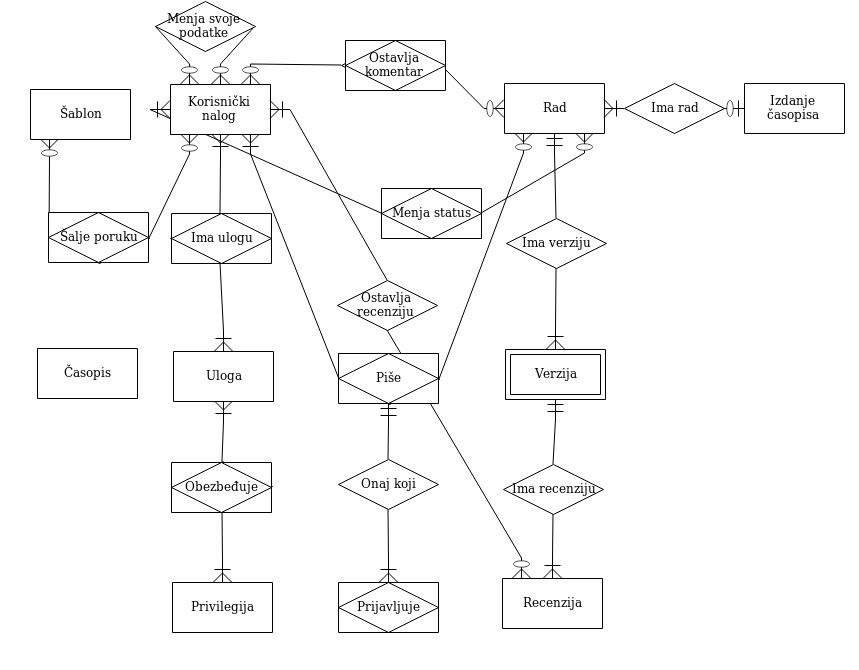
\includegraphics[width=\linewidth]{ERDiagram.png}
    \caption{ER dijagram}
    \label{fig:my_label}
\end{figure}

\begin{figure}[hbt!]
    \centering
    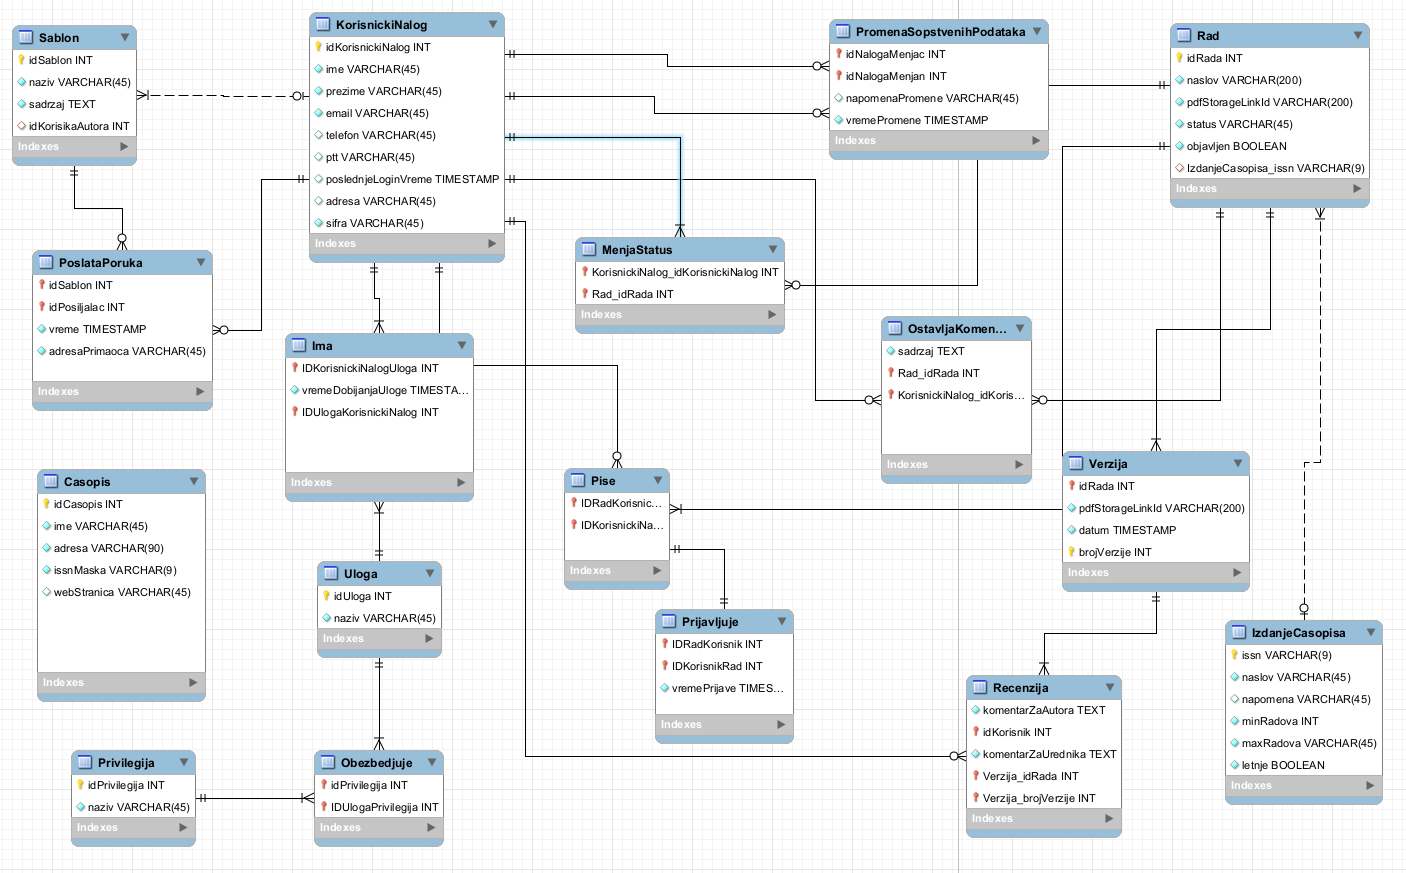
\includegraphics[width=\linewidth]{EER.png}
    \caption{EER dijagram}
    \label{fig:my_label}
\end{figure}

\end{document}
